\begin{mdframed}[style=warning]
	\begin{ejercicio}
		\textbf{Conceptos.}
		\begin{enumerate}
			\item ¿El velocímetro de un automóvil mide rapidez o velocidad?
			\item La parte superior de la figura (1) miestra una serie de fotografías de alta rapidez de un insecto que vuela en línea recta de izquierda a derecha. ¿Cuál de las gráficas mostradas describe el movimiento del insecto?
			 \begin{figure}[H]
			 	\centering
			 	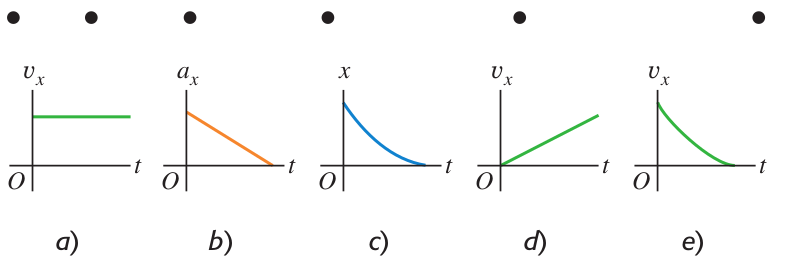
\includegraphics[scale=0.3]{./img/mosca.png}
			 	\caption{}
			 	\label{mosca}
			 \end{figure}
		\end{enumerate}
	\end{ejercicio}
\end{mdframed}





\begin{mdframed}[style=warning]
	\begin{ejercicio}
		El tiempo de Planck ($t_p$) es considerado como el intervalo de tiempo más pequeño que puede ser medido. En cosmología, el tiempo de Planck representa el instante más pequeño en el que las leyes de la física se pueden utilizar para estudiar la naturaleza. El tiempo de Planck se determina como combinación de otras constantes físicas en la siguiente forma:
			$$ t_p = \sqrt{\frac{\hbar G}{c^5}}. $$
		Utilizando las constantes fundamentales de la naturaleza
			\begin{table}[H]
				\centering
				\begin{tabular}{||c|c|c|c||}
					\hline
					\hline
						Símbolo & Nombre & Valor & Unidades \\
					\hline
					\hline
						$\hbar$ & Constante de Planck Reducida & $1.05457181\times 10^{-34}$ & $J\cdot s$ \\
						$G$ & Constante de Gravitación Universal & $6.674\times 10^{-11}$ & $N\cdot m^2 /kg^2$ \\
						$c$ & Velocidad de la luz en el vacío & $2.99792\times 10^8$ & $m/s$ \\
						$k_b$ & Constante de Boltzmann & $1.380649\times 10^{-23}$ & $J/K$ \\
					\hline
					\hline
				\end{tabular}
				\label{tabla}
			\end{table}
		Y sabiendo que las dimensionales de Joule y Newton se pueden expresar como: $[J] = [kg\cdot m^2 \cdot s^{-2}]$ y $[N] = [kg\cdot m\cdot s^{-2}]$. Por medio de análisis dimensional, encuentre las respectivas expresiones para la longitud de Planck, la masa de Planck, la energía de Planck y la temperatura de Planck.
	\end{ejercicio}
\end{mdframed}






\begin{mdframed}[style=warning]
	\begin{ejercicio}
		El conductor de un automóvil aplica los frenos cuando ve un árbol que bloquea el camino. El automóvil frena uniformemente con una aceleración de $5.6m/s^2$ durante $4.2s$, y hace marcas de derrape rectas de $62.4m$ de largo que terminan en el árbol. ¿Con qué rapidez el automóvil golpea el árbol?
	\end{ejercicio}
\end{mdframed}






\begin{mdframed}[style=warning]
	\begin{ejercicio}
		Una persona conduce su vehículo con rapidez constante de $15m/s$ y  pasa por un cruce escolar, donde el límite de velocidad es de $10m/s$. En ese preciso momento, un oficial de policía en su motocicleta, que está detenido en el cruce, arranca para perseguir al infractor, con aceleración constante de $3m/s^2$. ¿Cuánto tiempo pasa antes de qeu el oficial de policía alcance al infractor? ¿A qué rapidez va el policía en ese instante? 
	\end{ejercicio}
\end{mdframed}







\begin{mdframed}[style=warning]
	\begin{ejercicio}
		El maquinista de un tren que se mueve a una velocidad $v_1$, advierte la presencia de un tren de carga a una distancia $d$ delante de el que se mueve en la misma vía y en la misma dirección a una velocidad más lenta $v_2$. Acciona los frenos e imprime en su tren una asceleración constante $a$. Demuestre que:
			$$ \text{si} \quad d > \frac{(v_1 - v_2)^2}{2a} \quad \text{no habrá colisión;} $$
			$$ \text{si} \quad d < \frac{(v_1 - v_2)^2}{2a} \quad \text{habrá colisión.} $$
	\end{ejercicio}
\end{mdframed}





























%%%